\chapter{Conexões entre neurônios}\label{cap:conexoes}
\section{Introdução}\label{sec:conexoes_intro}

\section{Sinapses}\label{sec:sinapses}
\begin{description}
	\item[Sinapse] Uma conexão entre duas células neuronais. Podem ser de dois tipos:
	\begin{description}
		\item[Sinapses elétricas] se dão a partir de uma junção entre as duas células, por onde íons podem passar, produzindo uma corrente sináptica proporcional à diferença entre os potenciais de membrana das duas células
		\item[Sinapses químicas] são conectadas através de um espaço entre as células, e a interação entre elas se dá pela liberação de neurotransmissores. Podem ser excitatórias, causando despolarização da célula pós-sináptica, ou inibitórias, causando hiperpolarização
	\end{description}
	\item[Neurotransmissor] Um elemento químico que se propaga no espaço entre dois neurônios, fazendo a comunicação entre eles. Os mais comuns associados aos neurônios corticais são o \textbf{glutamato}, que excita a célula pós-sináptica, e o \textbf{ácido $\gamma$-aminobutírico (GABA)}, que a inibe
	\item[Neurônio pré-sináptico] O neurônio que libera o neurotransmissor durante a sinapse após o potencial de ação
	\item[Neurônio pós-sináptico] O neurônio que responde à liberação do neurotransmissor após o potencial de ação do neurônio pré-sináptico
	\item[Vesículas] Compartimentos ao redor da membrana neuronal por onde os neurotransmissores são transportados
\end{description}

\begin{figure}[htb!]
	\centering
	\caption{Esquema simplificado de uma sinapse química}
	\label{fig:sinapses}
	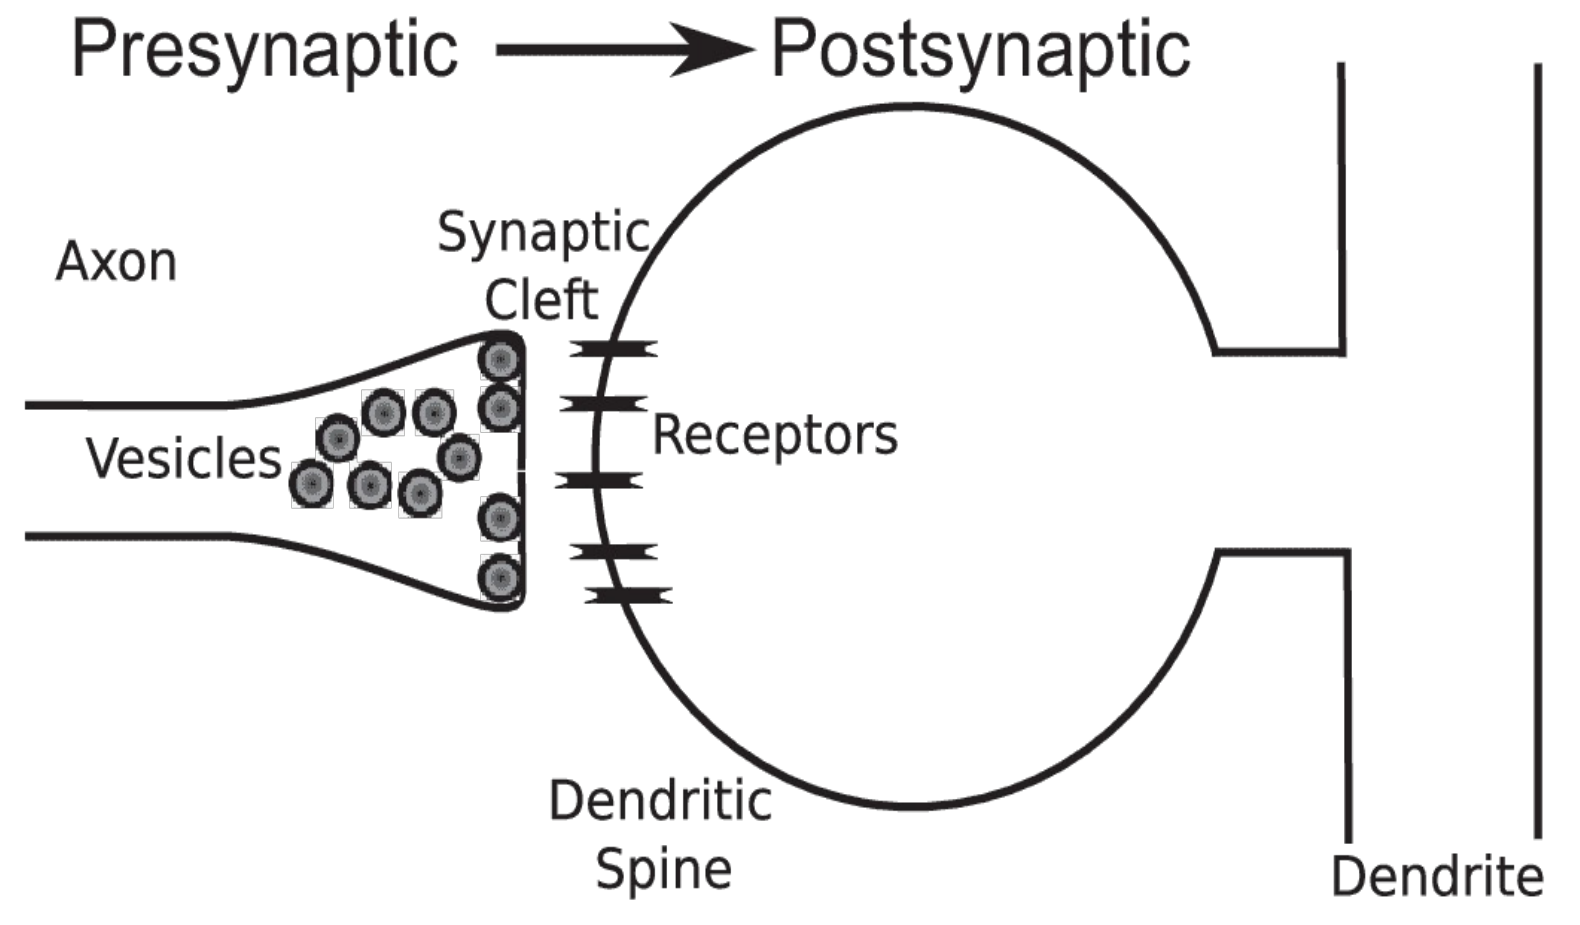
\includegraphics[width=0.7\linewidth]{figs/sinapses}
	\small{Fonte: \cite{miller_introductory_2018}}
\end{figure}


\subsection{Modelagem da transmissão sináptica}
\cite{dayan_theoretical_2001}
O modelo usado é:
$$
\frac{dG_{sin}(t)}{dt}=\frac{-G_{sin}(t)}{\tau_{sin}}
$$
sendo $G_{sin}(t)$ a condutância sináptica e $\tau_{sin}$ a constante de tempo específica para o tipo de sinapse. Além disso, se houver disparo da célula pré-sináptica, ocorre o seguinte mapeamento:
$$
G_{sin}(t)\mapsto G_{sin}(t)+\Delta G
$$
onde $\Delta G$ é o incremento de condutância. Um modelo mais elaborado considera o crescimento e decaimento de condutância usando a equação abaixo:
$$
\Delta G_{sin}(t)=\frac{\Delta G}{K}e^{-(t-t_{disparo})/\tau_{decai}}\Big[1-e^{-(t-t_{disparo})/\tau_{cresce}}\Big]
$$
com $\tau_{cresce}$ a constante de crescimento, $\tau_{decai}$ a constante de decaimento ($\tau_{decai}>\tau_{cresce}$), $t_{disparo}$ o instante do disparo da célula pré-sináptica, e $K$ um fator para garantir que a condutância tenha um valor máximo igual a $\Delta G$, dada por:
$$
K=\Bigg(\frac{\tau_{decai}}{\tau_{cresce}+\tau_{decai}}\Bigg)\Bigg(\frac{\tau_{cresce}}{\tau_{cresce}+\tau_{decai}}\Bigg)^{\tau_{cresce}/\tau_{decai}}
$$

\begin{figure}[htb!]
	\centering
	\caption{Condutância sináptica em resposta aos potenciais de ação da célula pré-sináptica}
	\label{fig:respostasinaptica}
	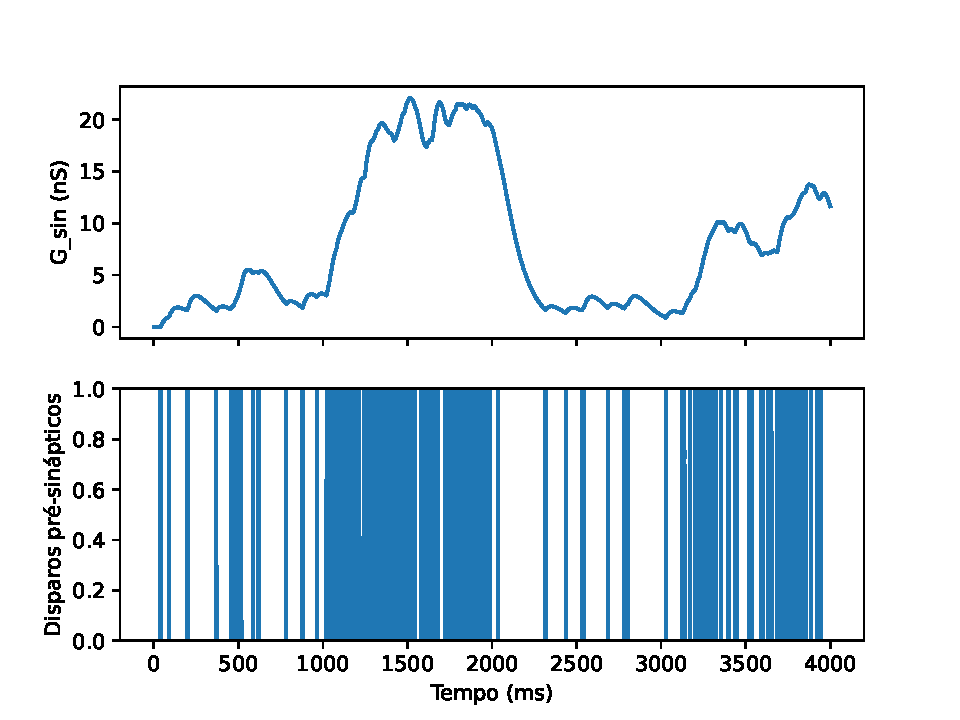
\includegraphics[width=0.8\linewidth]{figs/resposta_sinaptica}
\end{figure}


\section{Sinapses dinâmicas}\label{sec:dinamicas}
\begin{description}
	\item[Sinapse dinâmica] Sinapse cuja força varia em um curto período de tempo
	\item[Depressão de curta duração] Uma redução temporária na força sináptica
	\item[Facilitação de curta duração] Um incremento temporário na força sináptica
\end{description}

A simulação de depressão e facilitação sinápticas é feita alterando-se o valor de $\Delta G$ acima para:
$$
\Delta G=G_{max}p_0FD
$$
com $G_{max}$ o valor máximo de condutância sináptica, $p_0$ a probabilidade de liberação do neurotransmissor, e $F$ e $D$ as variáveis de facilitação e depressão sináptica, atualizadas por:
$$
\frac{dD}{dt}=\frac{1-D}{\tau_D}
$$$$
\frac{dF}{dt}=\frac{1-F}{\tau_F}
$$
e, seguindo cada disparo da célula pré-sináptica:
$$
D\mapsto D-p_0FD\qquad F\mapsto F+f_{fat}(F_{max}-F)
$$
com $F_{max}$ o valor máximo de facilitação e $F_{fat}$ denota o grau de facilitação ($0\leq f_{fat}\leq 1$)

%% falar da bomba de sódio e potassio ao falar do potencial de membrana

\section{Biestabilidade e \textit{feedback} recorrente}\label{sec:biestabilidade}

\subsection{Oscilações e multi-estabilidade}
\begin{description}
	\item[Bi-estabilidade] A capacidade dos neurônios de manter dois estados de atividades mesmo recebendo valores idênticos de entrada
	\item[Oscilações sublimiares] Variações no potencial de membrana insuficientes para a produção de um potencial de ação
	%\item[Quebra do anôdo] Um disparo no potencial de membrana que ocorre logo após uma hiperpolarização
	\item[Ressonância] Uma melhora na resposta de um sistema quando este é estimulado periodicamente com uma frequência particular
\end{description}

\begin{figure}[htb!]
	\centering
	\caption{Comportamento variado do modelo de Hodgkin-Huxley}
	\label{fig:hhdinamico}
	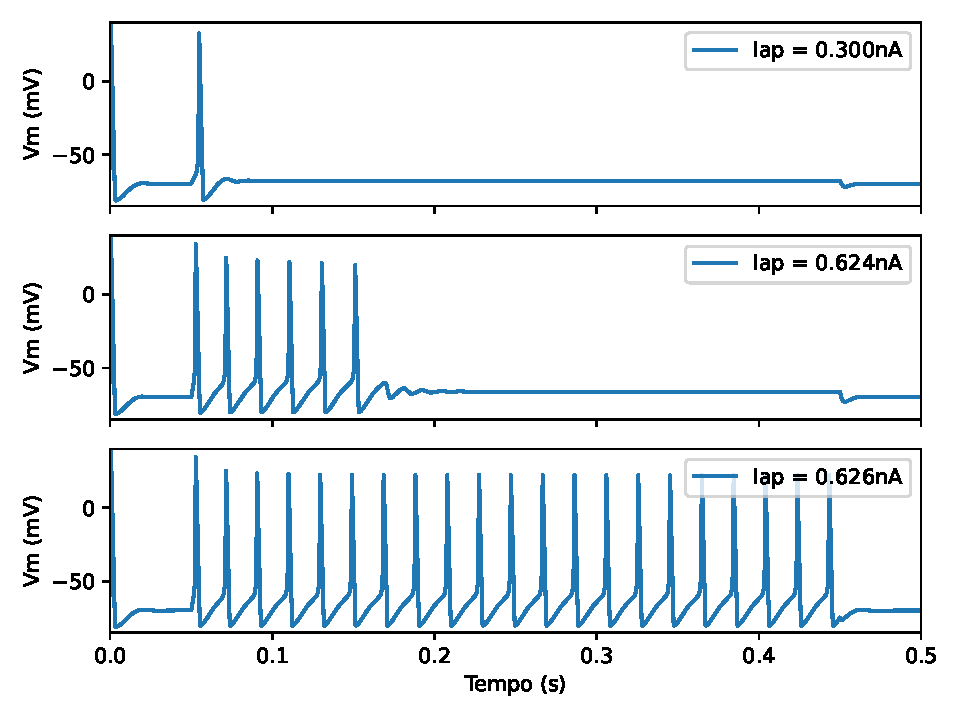
\includegraphics[width=0.7\linewidth]{figs/hh_dinamico}
\end{figure}
% a imagem daqui, das percepções de biestabilidade, está mais para a frente


\begin{description}
	\item[Unidade] Um grupo de neurônios cuja atividade média é simulada
	\item[Feedkback recorrente] Entrada de uma unidade que depende da sua própria atividade
\end{description}

% a imagem ta depois


\subsection{Geradores de padrão central}

\subsection{Circuitos tomadores de decisão}

\section{Caos e criticalidade}\label{sec:caos}
% colocar introdução
% transição de estados
% matemática dos estados

\subsection{Nullclines}
\begin{description}
	% isóclina de inclinação nula
	\item[Fase-plano] \textit{Plots} dos eixos das duas variáveis em um sistema de duas equações diferenciais ordinárias. Mostram os pontos fixos, \textit{nullclines} e trajetórias das variáveis ao longo do tempo
	\item[\textit{Nullcline} (Isóclina de inclinação nula)] Curvas que mostram a dependência de pontos fixos entre as variáveis de um sistema de equações diferenciais ordinárias. Cada equação diferencial gera uma \textit{nullcline}, e as interseções entre elas definem os pontos fixos do sistema
	%\item[Quebra do anôdo] Um disparo no potencial de membrana que ocorre logo após uma hiperpolarização
	\item[Pontos fixos] Pares de valores onde o sistema não se altera (o lado direito da equação diferencial ordinária é igual a 0)
\end{description}

% exemplo lotka-volterra
\begin{figure}[htb!]
	\centering
	\caption{\textit{Nullclines} em sistemas de Lotka-Volterra}
	\label{fig:nullclineslotkavolterra}
	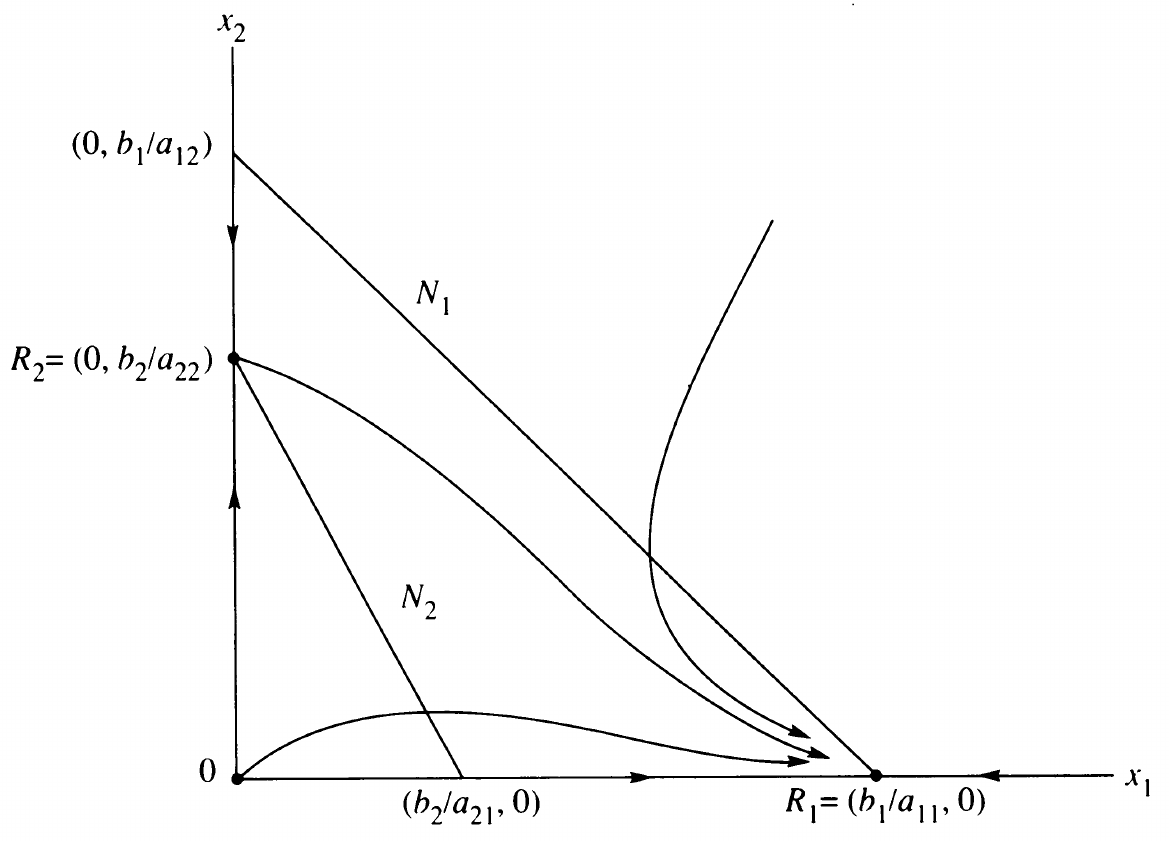
\includegraphics[width=0.7\linewidth]{figs/nullclines_lotka_volterra}\\
	\small{Fonte: \cite{zeeman_extinction_1995}}
\end{figure}

% exemplo fitz-hugh nagumo
\begin{figure}[htb!]
	\centering
	\caption{Plano de fase e estados fisiológicos no modelo FitzHugh-Nagumo}
	\label{fig:fitzhugh}
	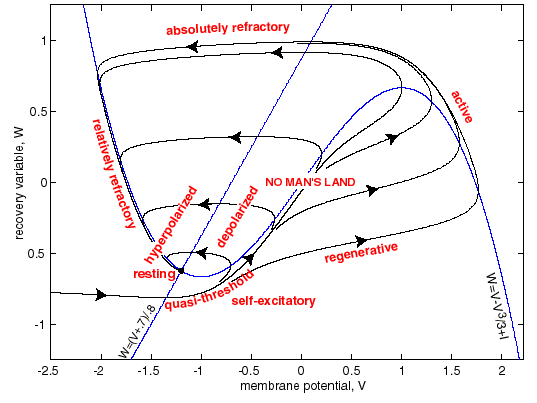
\includegraphics[width=0.7\linewidth]{figs/fitzhugh}\\
	\small{Fonte: Scholarpedia}
\end{figure}

% exemplo izhikevich
% exemplo livro (sistemas bi-estáveis)
\begin{figure}[htb!]
	\centering
	\caption{\textit{Nullclines} mostrando pontos fixos de sistemas bi-estáveis. A linha pontilhada é para $r_2$, e a contínua é para $r_1$. Os pontos fixos, onde as linhas se interceptam, são representados pelos círculos. Os sólidos são pontos estáveis, enquanto os abertos são instáveis.}
	\label{fig:nullcline}
	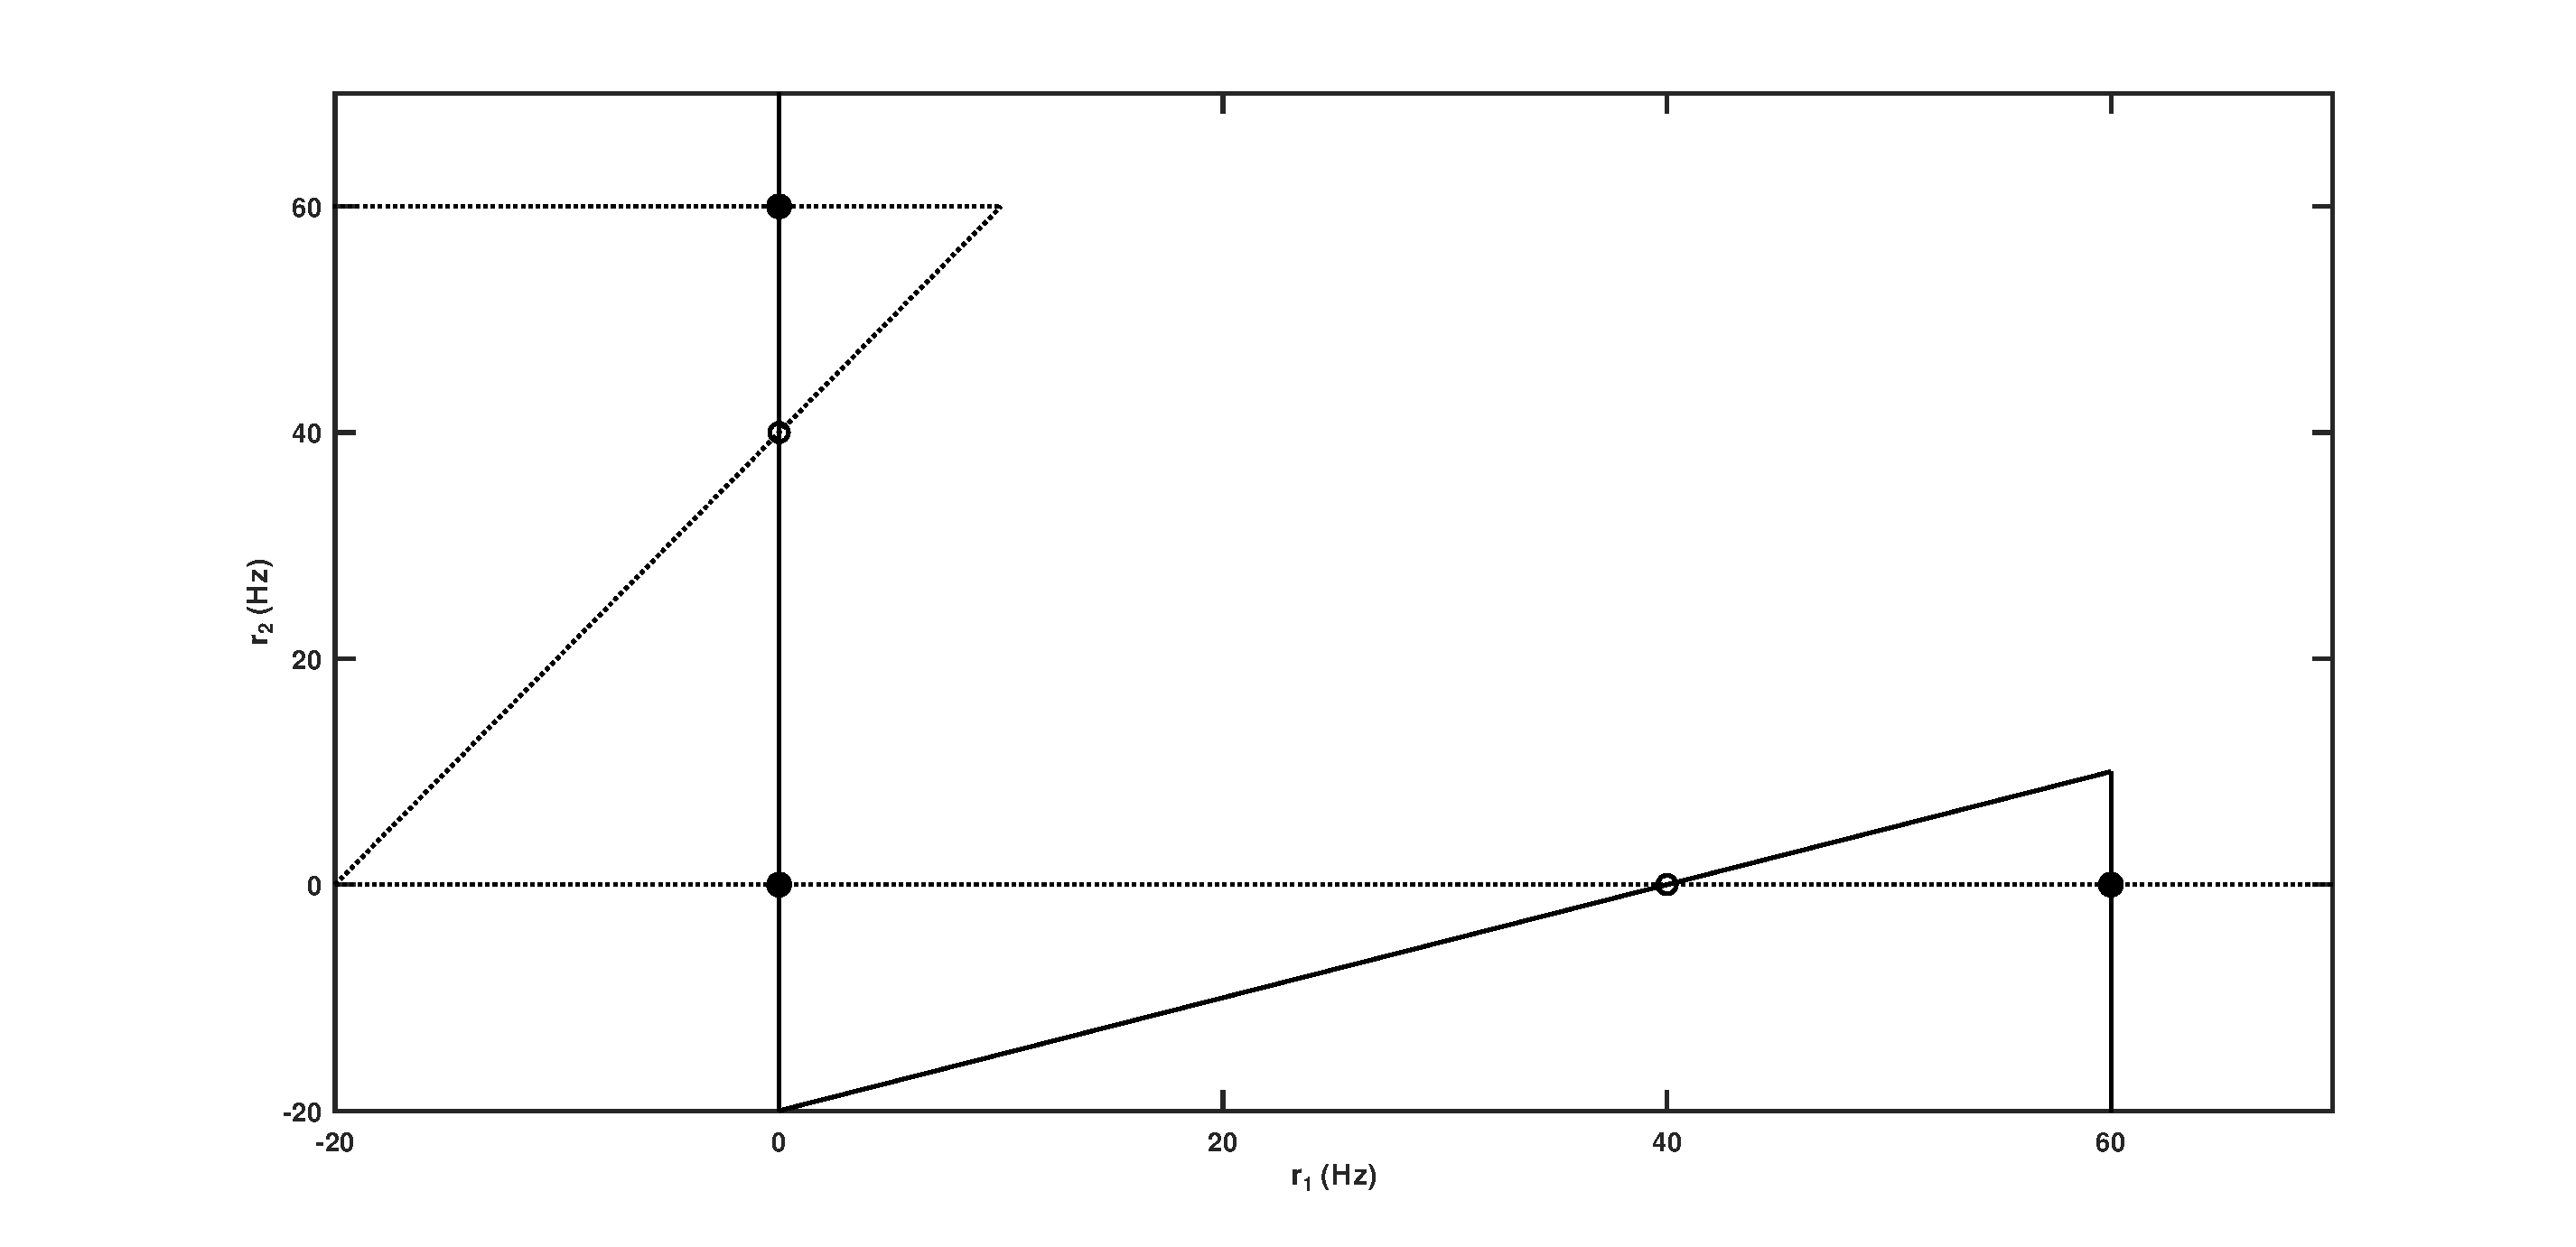
\includegraphics[width=0.9\linewidth]{figs/nullcline}\\
	\small{Fonte: adaptado de \cite{miller_introductory_2018}}
\end{figure}


\subsection{Estados atratores}
\begin{description}
	\item[Intinerância de estados atratores] A mudança de um sistema de um ponto fixo para outro
	\item[Rivalidade perceptual] Estímulos únicos podem ser percebidos de mais de uma maneira, alterando entre cada um dos perceptos (percepções bi-estáveis)
\end{description}

\begin{figure}[]
	\centering
	\caption{Imagens produzindo percepções de bi-estabilidade}
	\label{fig:biestabilidade}
	\begin{subfigure}[htb!]{0.3\textwidth}
		\caption{O cubo de Necker pode ser visto com a face frontal em lugares diferentes}
		\label{fig:cubonecker}
		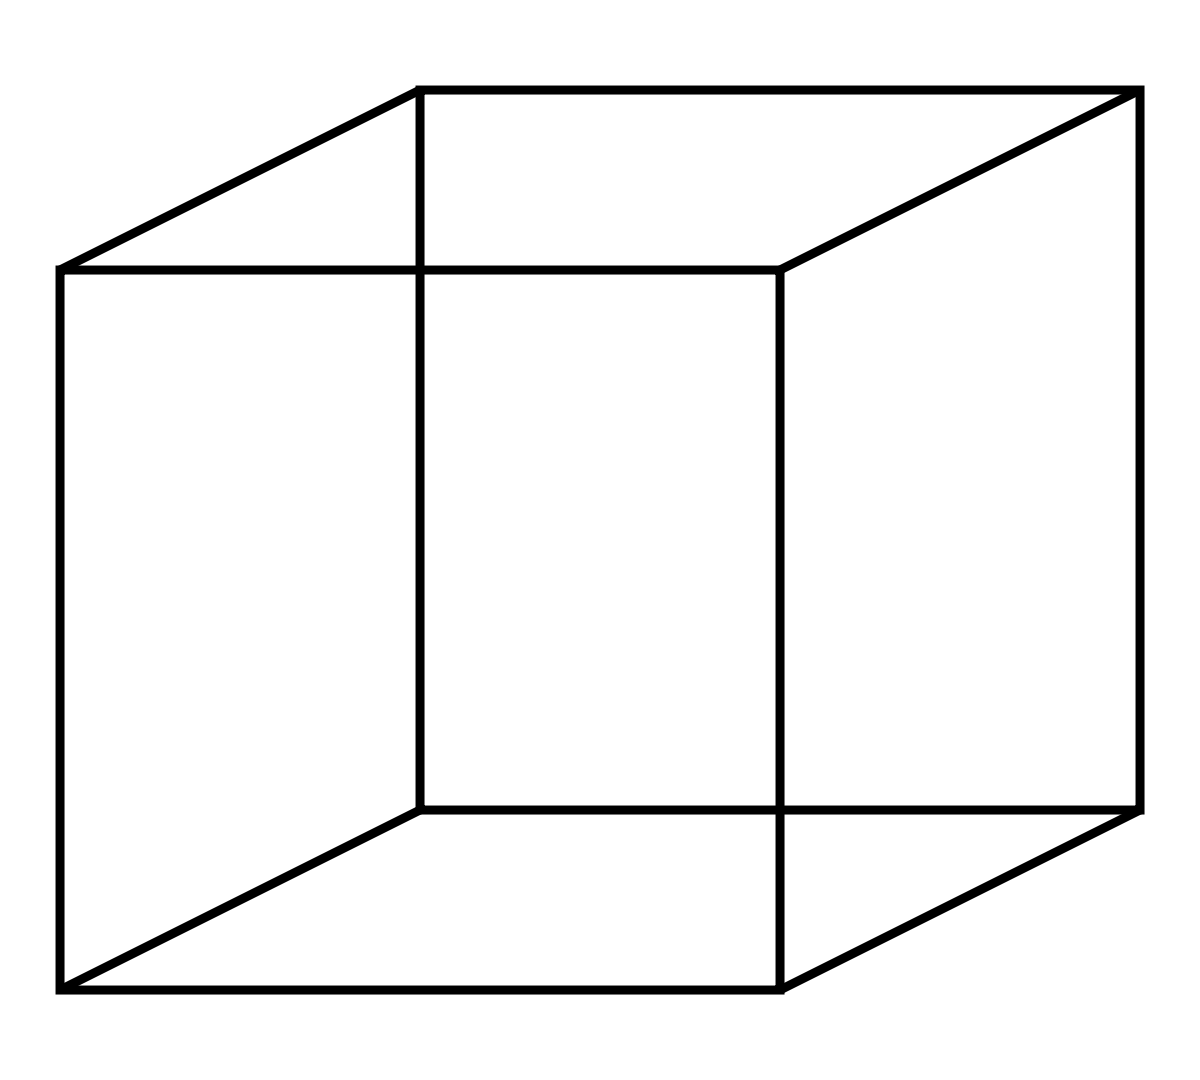
\includegraphics[width=\textwidth]{figs/cubo_necker}
	\end{subfigure}
	\qquad\qquad\qquad
	\begin{subfigure}[htb!]{0.3\textwidth}
		\caption{A imagem se assemelha tanto com um cão de frente quanto um homem de costas}
		\label{fig:vasorubin}
		
\includegraphics[width=0.8\textwidth]{figs/cao_homem}
	\end{subfigure}
\end{figure}


% indicar o estímulo
\begin{figure}[htb!]
	\centering
	\caption{Unidades de disparo com \textit{feedback} recorrente. A atividade média dos neurônios é simulada, e a saída da unidade também serve como entrada para a mesma. A força da conexão recorrente é excitatória, reforçando a taxa de disparos}
	\label{fig:feedbackrecorrente}
	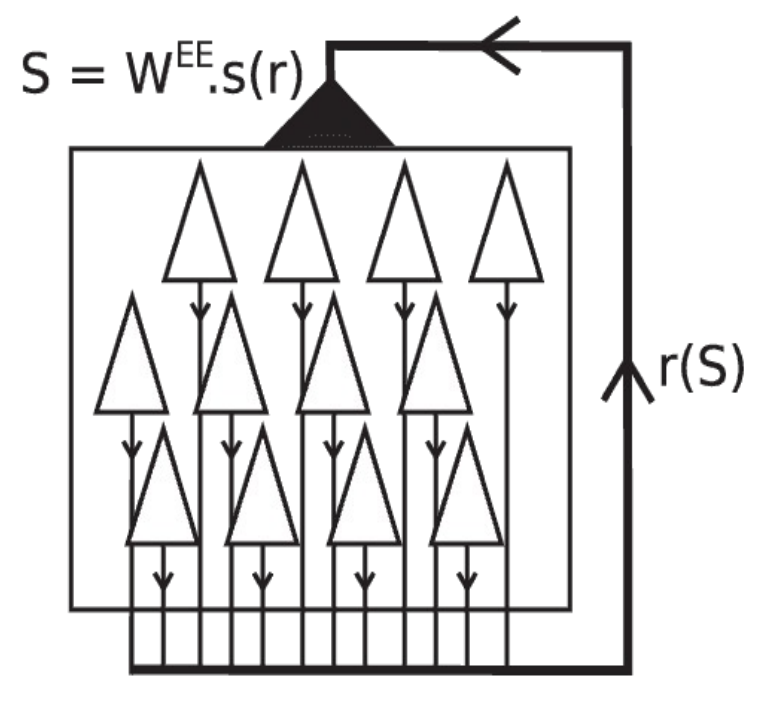
\includegraphics[width=0.45\linewidth]{figs/feedback_recorrente}
\end{figure}
sendo $r(S)$ a taxa média de disparos dos neurônios da unidade, que é função da entrada sináptica total, $S$, da fração de canais sinápticos abertos, $s(r)$, variável entre 0 e 1, multiplicado pela força de feedback, $W^{EE}$, o $EE$ indicando que é um feedback excitatório.
% ligar ambas as figuras
\begin{figure}[ht!]
	\centering
	\caption{Unidade com feedback recorrente que determina a estabilidade de um circuito. A taxa de disparo da unidade é uma função sigmoidal, a linha contínua na direita, e o feedback é representado pela linha tracejada. Na direita, a dinâmica da taxa de disparos em função do tempo, com um pulso de entrada entre 0,5 e 0,55 segundos (a região cinza). O feedback, nesse caso, é médio ($W^{EE}=0.6$), onde taxas baixas e altas de estado são estáveis, causando uma transição entre os estados do sistema}
	\label{fig:biestavel}
	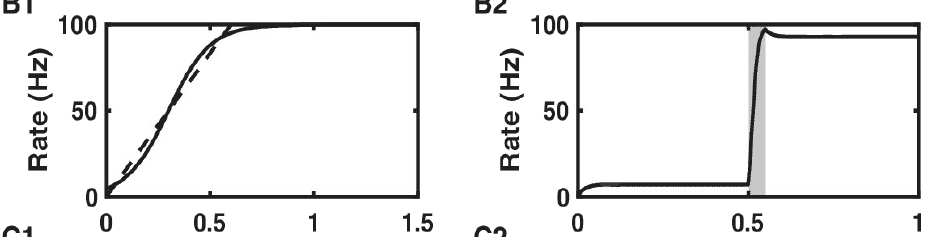
\includegraphics[width=0.7\linewidth]{figs/biestavel}
\end{figure}


\begin{figure}[htb!]
	\centering
	\caption{Unidades de decisão com feedback recorrente e interconexão. As conexões recorrentes são excitatórias, enquanto as interconexões são inibitórias. A presença de ruído, tanto na entrada quanto nas unidades, pode induzir a transições entre estados bi-estáveis}
	\label{fig:unidadesdecisao}
	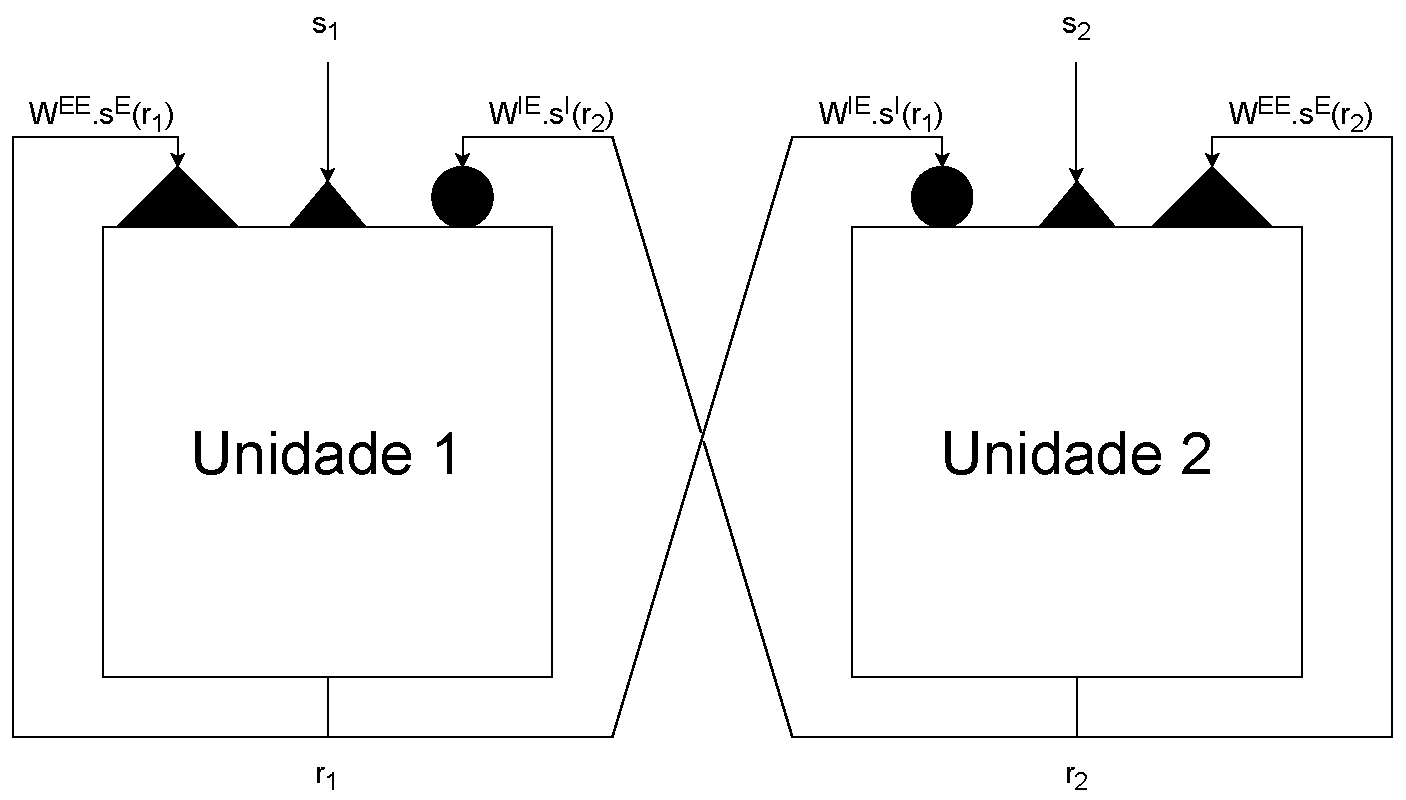
\includegraphics[width=0.7\linewidth]{figs/unidades_decisao}
\end{figure}

\begin{figure}[htb!]
	\centering
	\caption{Transições induzidas por ruído geram intinerância entre dois estados atratores, explicando alternância perceptual. Em (a), três \textit{trials} separados indicando alteração entre os estados, onde a atividade de uma unidade domina sobre a outra. Em (b), a média das atividades ao longo de 10 \textit{trials} (promediação)}
	\label{fig:noiseinducedtransitions}
	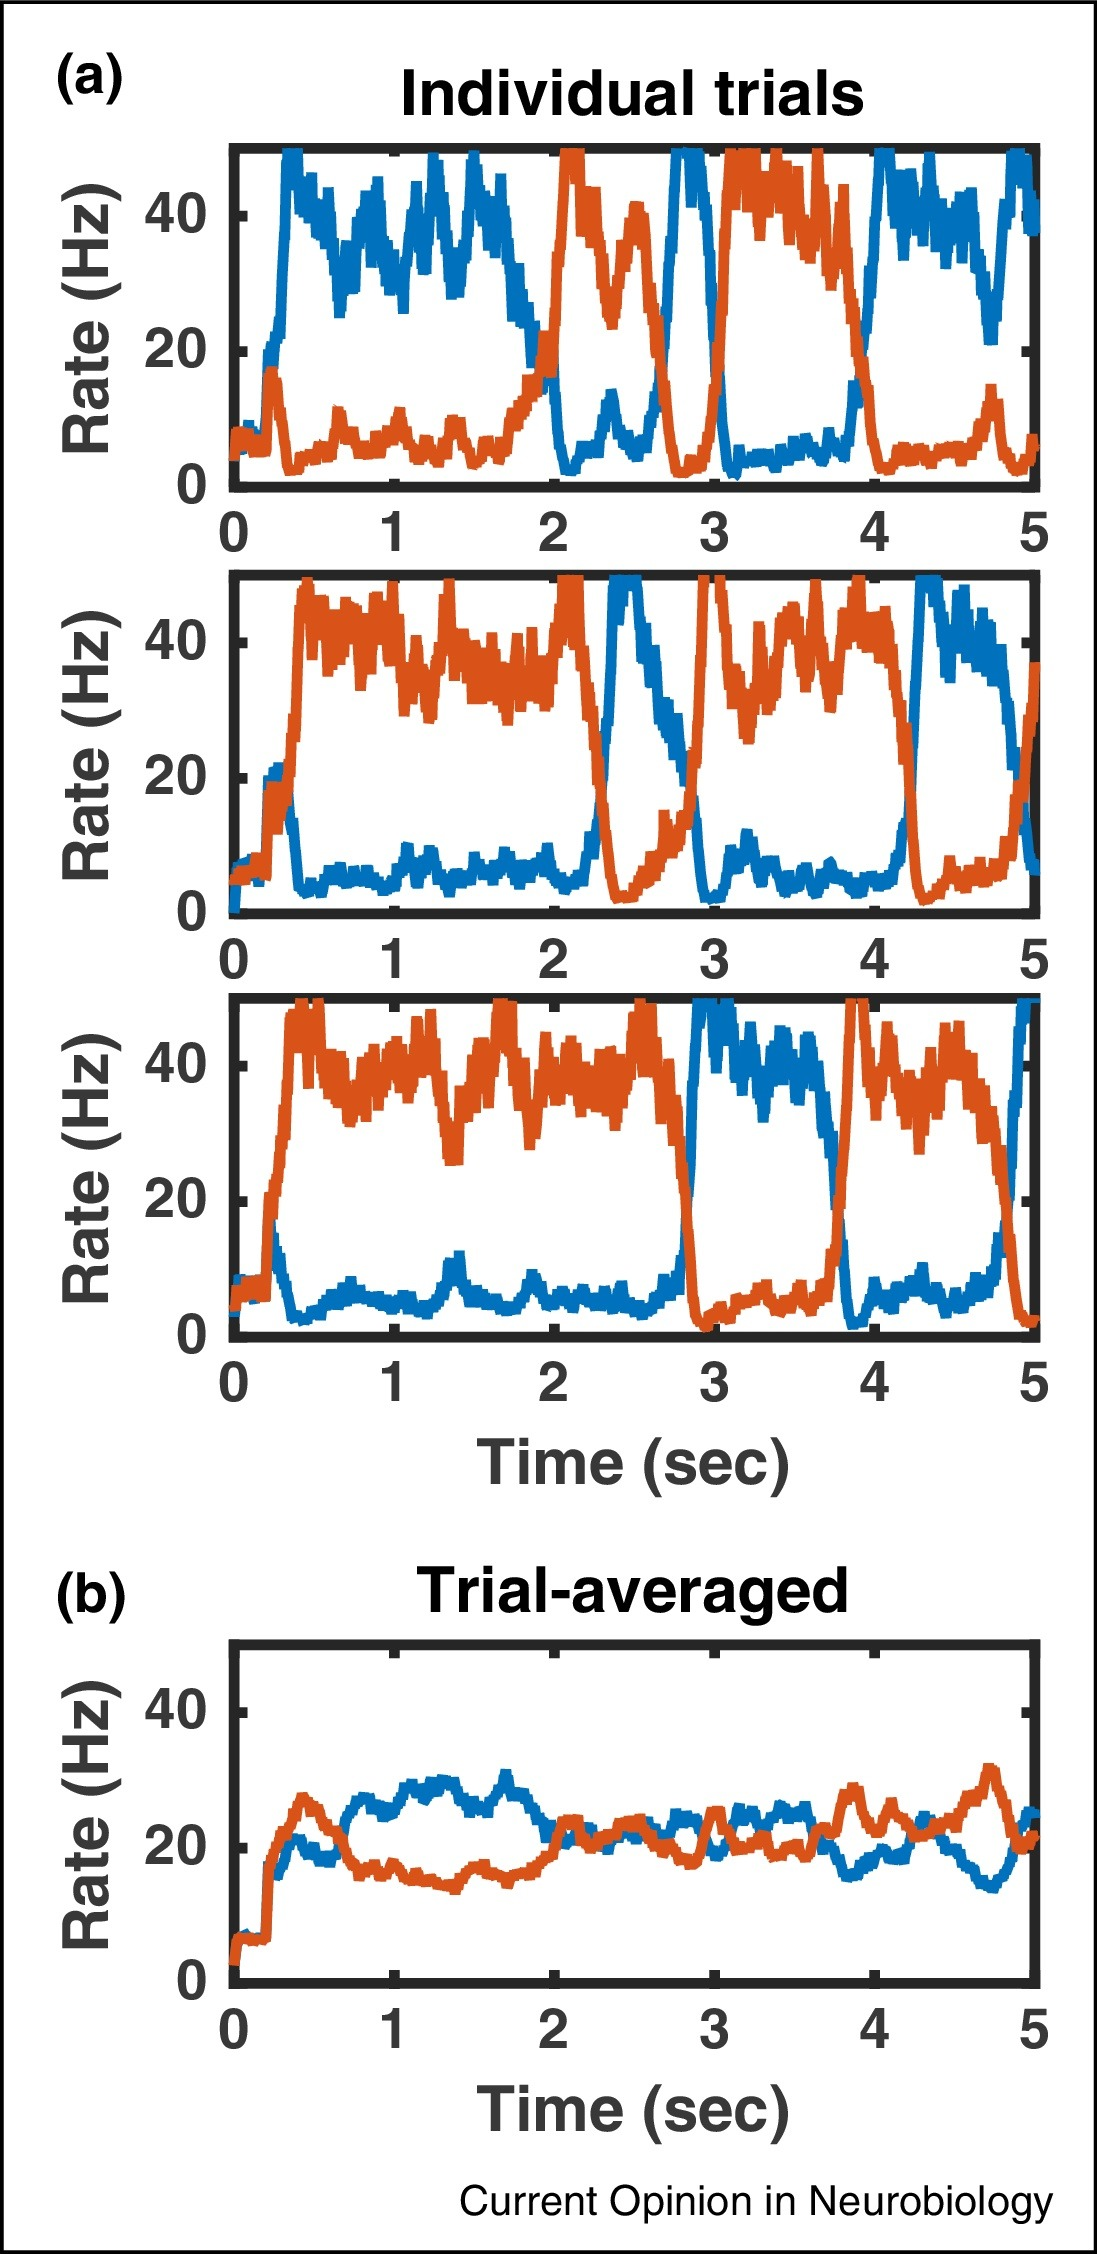
\includegraphics[width=0.35\linewidth]{figs/noise_induced_transitions}
\end{figure}


\subsubsection{Múltiplos atratores}
\begin{itemize}
	\item Alterações para mais de dois estados perceptuais
	\item Podem ser representados usando modelos ocultos de Markov (HMM, \textit{Hidden Markov Models})
	\item Na Figura~\ref{fig:hmm}, em (b), são mostrados os estados discretos que o HMM pode assumir nesse caso (círculos coloridos), com as matrizes de probabilidades de transição entre estados por unidade (a espessura das setas).
	\item Cada estado é definido pela probabilidade de emissão de um padrão particular em um intervalo de tempo (histogramas dentro dos círculos)
\end{itemize}

\begin{figure}[htb!]
	\centering
	\caption{Modelos ocultos de Markov. Em (a), os conjuntos de trens de disparo de potenciais de ação. Em (b), os estados discretos que o HMM assume. Em (c), as probabilidades a posteori para cada estado}
	\label{fig:hmm}
	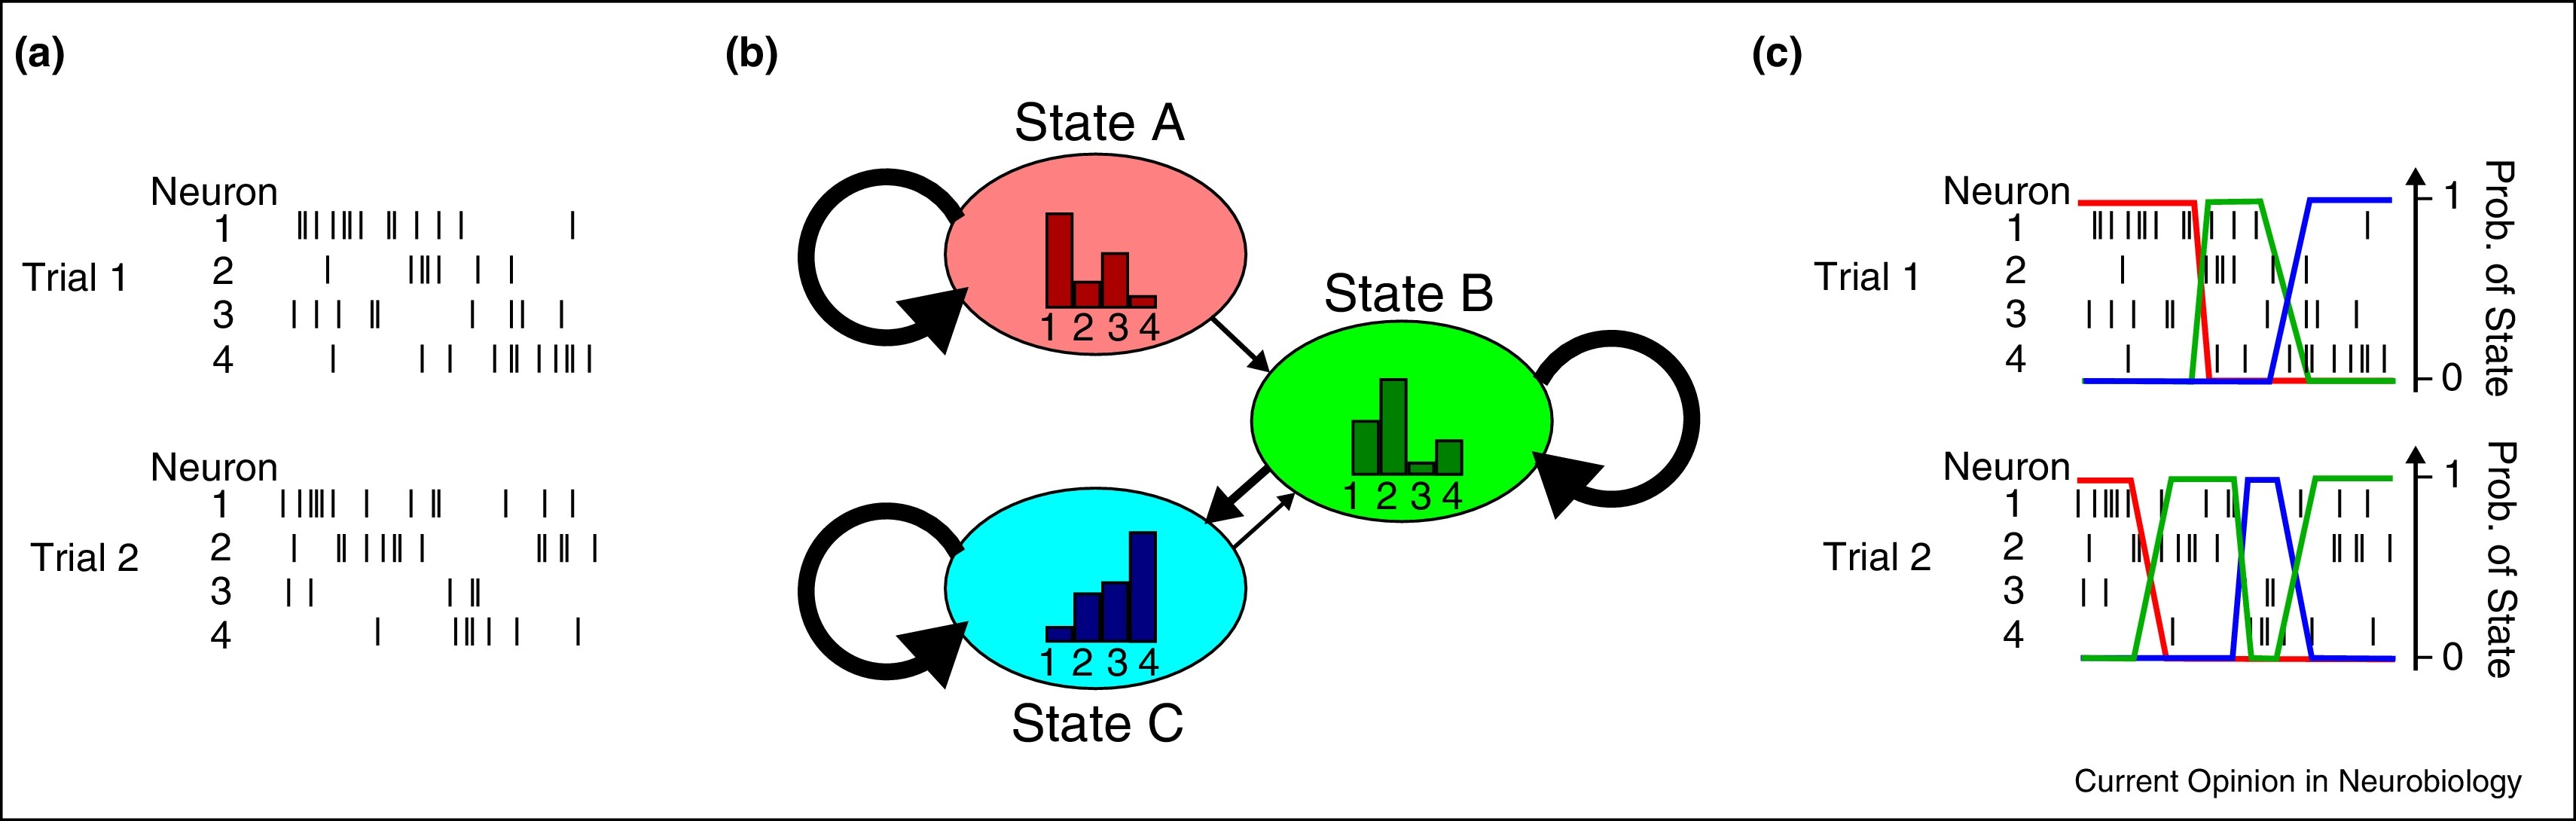
\includegraphics[width=0.8\linewidth]{figs/hmm}
\end{figure}


\subsection{Caos}
\begin{itemize}
	\item A \textbf{teoria do caos} é um ramo da matemática que lida com sistemas dinâmicos não lineares, ou seja, a interação dos componentes do sistema não é somente a adição desses componentes individualmente, devido a existência de efeitos multiplicativos ou de \textit{feedback}
	\item Sistemas caóticos podem ter poucas partes e seguirem regras bem simples, porém possuem uma sensibilidade bem grande às condições iniciais, onde o impacto de um pequeno efeito pode crescer exponencialmente ao longo do tempo
	\item A dinâmica não-linear de sistemas com caos facilita a habilidade de adaptação presente em sistemas neuronais, causando transições de um padrão de comportamento para outro quando o ambiente é alterado e, consequentemente, criando uma rica variedade de padrões
	\item Sistemas operam na \textbf{beira do caos} quando, para um mesmo conjunto de parâmetros, se ajustados em uma direção tornam o sistema caótico, enquanto que se ajustados em outra direção fazem com que o sistema apresente estados estáveis
	\item O conjunto de parâmetros, na condição de beira do caos, pode ser chamado de crítico, com o sistema podendo exibir \textbf{criticalidade}, uma propriedade dos sistemas onde uma pequena alteração do sistema em um local pode tanto ter um efeito local quanto se propagar e alterar o sistema como um todo
	\item Acredita-se que sistemas em criticalidade possuem melhores capacidades de processamento de informação e otimização de memória, inspirando a hipótese da criticalidade, proposição onde o cérebro opera em um estado crítico, devido às capacidades de computação ótimas associadas precisarem ser evolutivamente selecionadas para isso
	\item A ideia geral de sistemas se auto migrarem para estados críticos através de processos descentralizados é conhecido como \textbf{criticalidade auto-organizável} (SOC, \textit{self-organized criticality})
	\item Uma cascata de disparos de atividade neuronal que ultrapassa um limiar em intervalos de tempo seguidos é chamado de \textbf{avalanche} (Fig.~\ref*{fig:sandpile})
	\item Exemplos de sistemas que podem exibir comportamento caótico incluem o modelo de neurônio de Izhikevich (já visto) e a equação do mapa logístico (tutorial), dada por $x_{t+1}=rx_t(1-x_t)$, e que representa um modelo discreto de crescimento populacional, sendo $x_t$ a taxa de população no tempo $t$ e $r$ a taxa de crescimento
\end{itemize}

\begin{figure}[htb!]
	\centering
	\caption{Modelo de pilha de areia}
	\label{fig:sandpile}
	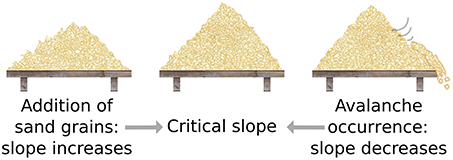
\includegraphics[width=0.7\linewidth]{figs/sandpile}
\end{figure}


%\subsection{Coeficiente de Lypunov}

%\subsection{Avalanches}
